\subsection*{A1. How to Install}
\dReach{} is an open source project under GPL-3 license. We bundled
\dReal{} and \dReach{} together and host them at
\url{http://dreal.github.io}. The BMC encoder module is written in
OCaml and uses Oasis and OCaml Batteries library. At the release
page\footnote{\url{http://dreal.github.io/download}}, we host
pre-compiled static-binaries for Linux and OS X, which do not require
any compilation to use \dReach{} in those platforms.

\subsection*{A2. Syntax Grammar of \drh{}}
\begin{align*}
  % drh
  \mathit{drh} \ := \ & \mathit{macro\_def}^* \
  \mathit{variable\_decl}^+ \ \mathit{mode\_def}^+ \  \mathit{initial\_cond} \  \mathit{goal}^+\\
  % variable-decl
  \mathit{macro\_decl} \ := \ &  \texttt{\#define} \ \mathit{var} \ (\mathit{expr} \, | \, \mathit{formula})\\
  % variable-decl
  \mathit{variable\_decl} \ := \ &  \texttt{[} \mathit{l} \texttt{,} \ \mathit{u} \texttt{]} \ \mathit{var} \texttt{;}\\
  % variable-decl
  \mathit{mode\_def} \ := \ & \texttt{\{}
  \texttt{mode} \
  \mathit{id}\texttt{;} \quad
  \texttt{invt}:(\mathit{formula} \texttt{;})^+ \ \ \
  \texttt{flow}:\mathit{ode}^+ \ \ \ \texttt{jump}:\mathit{jump}^+ \texttt{\}}\\
  \mathit{ode} \ := \ & \texttt{d/dt[}\mathit{x}\texttt{]=}\mathit{exp}\\
  \mathit{jump} \ := \ & \mathit{formula} \ \texttt{==>} \ \texttt{@}\mathit{n} \ \mathit{formula}\\
  \mathit{initial\_cond} \ := \ & \texttt{@}\mathit{mode\_id} \ \mathit{formula}\texttt{;}\\
  \mathit{goal}              \ := \ & \texttt{@}\mathit{mode\_id} \ \mathit{formula}\texttt{;}
\end{align*}
Note that we use the standard definitions for $\mathit{formlua}$ and
$\mathit{expr}$ here.

\subsection*{A3. An Example of Encoded SMT2 Formula}

\paragraph{Example encoding} The bounded reachability problem of a
bouncing ball example (when $k = 3$) is encoded into the following
shortened SMT2 formula.
\begin{Verbatim}[fontfamily=courier, frame=single, framesep=1mm,  numbers=left, fontsize=\scriptsize]
(set-logic QF_NRA_ODE)
(declare-fun x_0_0 () Real) ...
(declare-fun v_0_t () Real) ...
(declare-fun time_0 () Real) ...
(define-ode flow_1 ((= d/dt[x] v)
                    (= d/dt[v] (+ (- 0.0 9.8) (* -0.45 (^ v 2.0))))))
(define-ode flow_2 ((= d/dt[x] v)
                    (= d/dt[v] (+ (- 0.0 9.8) (* +0.45 (^ v 2.0))))))
(assert (<= 0.0 x_0_0)) ...
(assert (<= v_10_t 18.0))
(assert (<= 0.0 time_0))
(assert (and (and (= v_0_0 0.0) (>= x_0_0 5.0)) (= mode_0 1.0) (=
[x_0_t v_0_t] (integral 0. time_0 [x_0_0 v_0_0] flow_1)) (= mode_0
1.0) (forall_t 1.0 [0.0 time_0] (<= v_0_t 0.0)) (<= v_0_t 0.0) (<=
...
x_9_t) (= [x_10_t v_10_t] (integral 0. time_10 [x_10_0 v_10_0]
flow_1)) (= mode_10 1.0) (forall_t 1.0 [0.0 time_10] (<= v_10_t 0.0))
(<= v_10_t 0.0) (<= v_10_0 0.0) (forall_t 1.0 [0.0 time_10] (>= x_10_t
0.0)) (>= x_10_t 0.0) (>= x_10_0 0.0) (= mode_10 1.0) (>= x_10_t
0.45))) (check-sat) (exit)
\end{Verbatim}


% Figure~\ref{fig:viz} is a screenshot of the
% visualization for a cardiac-cell model.
% \begin{figure}
%   \centering
%   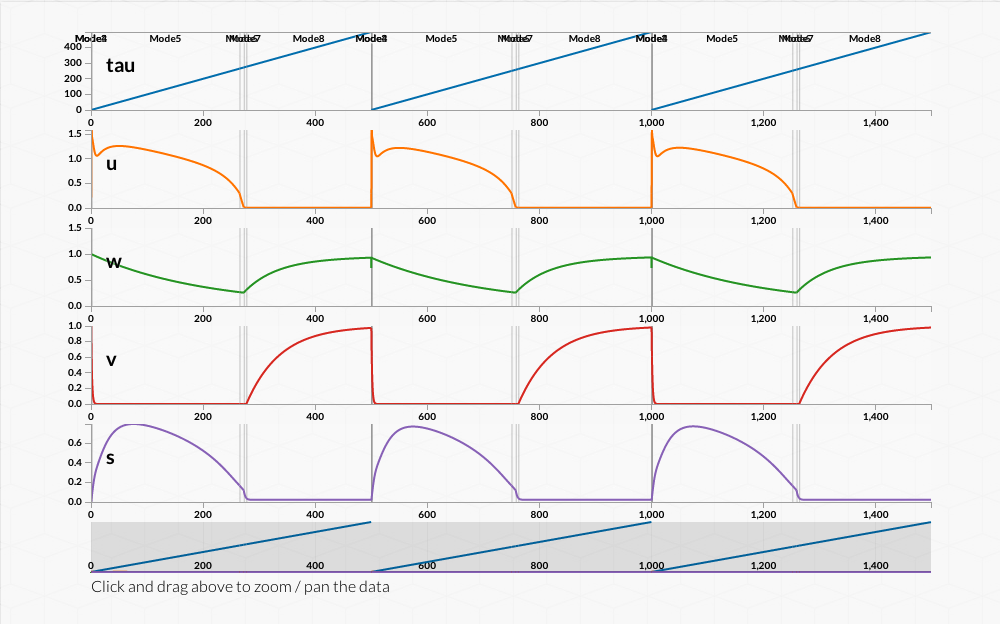
\includegraphics[width=\textwidth]{images/cardiac}
%   \caption{Visualization of $\delta$-reachable trajectory for
%     a cardiac-cell model.}
%   \label{fig:viz}
% \end{figure}

\subsection*{A4. Experiments}\label{sec:exp}

% Our tool \dReach{} implements the techniques presented in the
% paper. The tool is built on several existing packages,including {\sf
%   opensmt}~\cite{DBLP:conf/tacas/BruttomessoPST10} for the general
% DPLL(T) framework, {\sf
%   realpaver}~\cite{DBLP:journals/toms/GranvilliersB06} for ICP, and
% {\sf CAPD}~\cite{capd} for computing interval-enclosures of ODEs. The
% tool is open-source at~\url{http://dreal.cs.cmu.edu/dreach.html}.

\newcommand{\hmodel}[2]{\href{http://dreal.cs.cmu.edu/#1}{#2}}
{\small
\begin{table}[!th]
  \centering
  \small
  \begin{tabular}{l|r|r|r|r|r|r|r|r}
    \hline
    \hline
    Benchmark    & \#Mode& \#Depth & \#ODEs & \#Vars  & Delta  & Result       & Time(s) & Trace \\
    \hline
    \hline
      AF-GOOD & 4     & 3        & 20     & 53      & 0.001     & SAT &  0.425    & 793K     \\
       AF-BAD & 4     & 3        & 20     & 53      & 0.001     & UNSAT &  0.074    & ---      \\
  AF-TO1-GOOD & 4     & 3        & 24     & 62      & 0.001     & SAT &  2.750    & 224K     \\
   AF-TO1-BAD & 4     & 3        & 24     & 62      & 0.001     & UNSAT &  5.189    & ---     \\
  AF-TO2-GOOD & 4     & 3        & 24     & 62      & 0.005     & SAT &  3.876    & 553K     \\
   AF-TO2-BAD & 4     & 3        & 24     & 62      & 0.001     & UNSAT &  8.857    & ---     \\
 AF-TSO1-TSO2 & 4     & 3        & 24     & 62      & 0.001     & UNSAT &  0.027    & ---     \\
       AF8-K7 & 8     & 7        & 40     & 101     & 0.001     & SAT & 10.478   & 3.8M      \\
      AF8-K23 & 8     & 23       & 40     & 293     & 0.001     & SAT & 135.29   & 11M      \\
    \hline
    \hline
    EO-K2  & 3     & 2        & 18     & 48      & 0.01    & SAT & 3.144    & 1.9M      \\
    EO-K11 & 3     & 11       & 99     & 174     & 0.01    & UNSAT & 0.969    & ---       \\
    \hline
    \hline
    QUAD-K1  & 2   & 1          & 34     & 89      & 0.01      & SAT & 2.386 &  10M \\
    QUAD-K2  & 2   & 2          & 34     & 125     & 0.01      & SAT & 4.971 &  13M \\
    QUAD-K3  & 4   & 3          & 68     & 161     & 0.01      & SAT & 13.755 & 42M \\
    QUAD-K3U & 4   & 3          & 68     & 161     & 0.01      & UNSAT & 2.846 & --- \\
    \hline
    \hline
    CT       & 2   & 2         & 10      & 41      & 0.005     & SAT & 345.84 & 3.1M\\
    CT       & 2   & 2         & 10      & 41      & 0.002     & SAT & 362.84 & 3.1M\\
    \hline
    \hline
    BB-K10 & 2     & 10       & 22     & 66      & 0.01        & SAT & 8.057     & 123K  \\
    BB-K20 & 2     & 20       & 42     & 126     & 0.01        & SAT & 39.196    & 171K  \\
    \hline
    \hline
  \end{tabular}
  \caption{\small
    Summary of the running time of the tool on various hybrid system
    models:
    \#Mode = Number of modes in the hybrid system,
    \#Depth = Unrolling depth,
    \#ODEs = Number of ODEs in the unrolled formula,
    \#Vars = Number of variables in the unrolled formula,
    Result = Bounded Model Checking Result (delta-SAT/UNSAT)
    Time = CPU time (s),
    Trace = Size of the ODE trajectory,
    AF = Atrial Filbrillation,
    EO = Electronic Oscillator,
    QUAD = Quadcopter Control,
    CT = Cancer Treatment,
    BB = Bouncing Ball with Drag.
    % TIMES = Solving time in seconds, TO = Timeout (30min), PC = Proof
    % Checked, #PA = Number of proved axioms, #SP = Number of subproblems
    % generated by proof checking, TIMEPC = Proof-checking time in seconds, #D =
    % Number of iteration depth required in proof checking
}\label{tbl:exp}
\end{table}


All benchmarks and data shown here are also available on the tool
website\footnote{\url{http://dreal.github.io}}. Due to space limit,
we only highlight the typical nonlinear differential equations in the
models. All models are hybrid systems with multiple modes containing
these equations All experiments were conducted on a machine with a
3.4GHz octa-core Intel Core i7-2600 processor and 16GB RAM, running
64-bit Ubuntu 12.04LTS. Table~\ref{tbl:exp} is a summary of the
running time of the tool on various hybrid system models.

\paragraph{Atrial Fibrillation.} We studied the Atrial Fibrillation model. The model has four discrete control locations, four state variables, and nonlinear ODEs. A typical set of ODEs in the model is:
\begin{eqnarray*}
\frac{du}{dt} &=& e + (u-\theta_v)(u_u-u ) v g_{fi} + wsg_{si}-g_{so}(u)\\
\frac{ds}{dt} &=& \displaystyle\frac{g_{s2}}{(1+\exp(-2k(u-us)))} -  g_{s2}s\\
\frac{dv}{dt} &=& -g_v^+\cdot v \hspace{1cm} \frac{dw}{dt} = -g_w^+\cdot w
\end{eqnarray*}
The exponential term on the right-hand side of the ODE is the sigmoid function, which often appears in modelling biological switches.

\paragraph{Prostate Cancer Treatment.} The Prostate Cancer Treatment model~\cite{CMSB14} exhibits more nonlinear ODEs. The reachability questions are
\begin{eqnarray*}
\frac{dx}{dt} &=& (\alpha_x
(k_1+(1-k_1)\frac{z}{z+k_2}-\beta_x( (1-k_3)\frac{z}{z+k_4}+k_3)) - m_1(1-\frac{z}{z_0}))x + c_1 x\\
\frac{dy}{dt} &=& m_1(1-\frac{z}{z_0})x+(\alpha_y (1- d\frac{z}{z_0}) - \beta_y)y+c_2y\\
\frac{dz}{dt} &=& \frac{-z}{\tau} + c_3z\\
\frac{dv}{dt} &=& (\alpha_x
(k_1+(1-k_1)\frac{z}{z+k_2}-\beta_x(k_3+(1-k_3)\frac{z}{z+k_4}))\\
& &- m_1(1-\frac{z}{z_0}))x + c_1 x + m_1(1-\frac{z}{z_0})x+(\alpha_y (1- d\frac{z}{z_0}) - \beta_y)y+c_2y
\end{eqnarray*}

\paragraph{Electronic Oscillator.} The EO model represents an electronic oscillator model that contains nonlinear ODEs such as the following:
\begin{eqnarray*}
\frac{dx}{dt} &=& - ax \cdot sin(\omega_1 \cdot \tau)\\
\frac{dy}{dt} &=& - ay \cdot sin( (\omega_1 + c_1) \cdot \tau) \cdot sin(\omega_2)\cdot 2\\
\frac{dz}{dt} &=& - az \cdot sin( (\omega_2 + c_2) \cdot \tau) \cdot cos(\omega_1)\cdot 2\\
\frac{\omega_1}{dt} &=& - c_3\cdot \omega_1\ \ \ \frac{\omega_2}{dt} = -c_4\cdot\omega_2\ \ \ \frac{d\tau}{dt} = 1
\end{eqnarray*}

\paragraph{Quadcopter Control.} We developed a model that contains the full dynamics of a quadcopter. We use the model to solve control problems by answering reachability questions. A typical set of the differential equations are the following:
\begin{eqnarray*}
\frac{\mathrm{d}\omega_x}{\mathrm{d}t} &=& L\cdot k\cdot (\omega_1^2 - \omega_3^2)(1/I_{xx})-(I_{yy} - I_{zz})\omega_y\omega_z/I_{xx}\\
\frac{\mathrm{d}\omega_y}{\mathrm{d}t} &=& L\cdot k\cdot(\omega_2^2 - \omega_4^2)(1/I_{yy})-(I_{zz} - I_{xx})\omega_x\omega_z/I_{yy}\\
\frac{\mathrm{d}\omega_z}{\mathrm{d}t} &=& b\cdot(\omega_1^2 - \omega_2^2 + \omega_3^2 - \omega_4^2)(1/I_{zz})-(I_{xx} - I_{yy})\omega_x\omega_y/I_{zz}\\
\frac{\mathrm{d}\phi}{\mathrm{d}t} &=& \omega_x + \displaystyle{\frac{\sin\left(\phi\right) \sin\left(\theta\right)}{{\left(\frac{\sin\left(\phi\right)^{2} \cos\left(\theta\right)}{\cos\left(\phi\right)} + \cos\left(\phi\right) \cos\left(\theta\right)\right)} \cos\left(\phi\right)}}\omega_y + \displaystyle\frac{\sin\left(\theta\right)}{\frac{\sin\left(\phi\right)^{2} \cos\left(\theta\right)}{\cos\left(\phi\right)} + \cos\left(\phi\right) \cos\left(\theta\right)}\omega_z\\
\frac{\mathrm{d}\theta}{\mathrm{d}t} &=& -(\displaystyle\frac{\sin\left(\phi\right)^{2} \cos\left(\theta\right)}{{\left(\frac{\sin\left(\phi\right)^{2} \cos\left(\theta\right)}{\cos\left(\phi\right)}\omega_y + \cos\left(\phi\right) \cos\left(\theta\right)\right)} \cos\left(\phi\right)^{2}} + \frac{1}{\cos\left(\phi\right)})\omega_y\\
& &\hspace{5cm}-\displaystyle\frac{\sin\left(\phi\right) \cos\left(\theta\right)}{{\left(\frac{\sin\left(\phi\right)^{2} \cos\left(\theta\right)}{\cos\left(\phi\right)} + \cos\left(\phi\right) \cos\left(\theta\right)\right)} \cos\left(\phi\right)}\omega_z \\
\frac{\mathrm{d}\psi}{\mathrm{d}t} &=& \displaystyle\frac{\sin\left(\phi\right)}{{\left(\frac{\sin\left(\phi\right)^{2} \cos\left(\theta\right)}{\cos\left(\phi\right)} + \cos\left(\phi\right) \cos\left(\theta\right)\right)} \cos\left(\phi\right)}\omega_y + \displaystyle\frac{1}{\frac{\sin\left(\phi\right)^{2} \cos\left(\theta\right)}{\cos\left(\phi\right)} + \cos\left(\phi\right) \cos\left(\theta\right)}\omega_z\\
\frac{\mathrm{d}{xp}}{\mathrm{d}t} &=& (1/m)(\sin(\theta)\sin(\psi)k(\omega_1^2 + \omega_2^2 +\omega_3^2+\omega_4^2) - k\cdot d\cdot{xp})\\
\frac{\mathrm{d}{yp}}{\mathrm{d}t} &=& (1/m)(-\cos(\psi)\sin(\theta)k(\omega_1^2 + \omega_2^2 +\omega_3^2+\omega_4^2) - k\cdot d\cdot{yp})\\
\frac{\mathrm{d}{zp}}{\mathrm{d}t} &=& (1/m)(-g-\cos(\theta)k(\omega_1^2 + \omega_2^2 +\omega_3^2+\omega_4^2) - k\cdot d\cdot{zp}\\
\frac{\mathrm{d}x}{\mathrm{d}t} &=& {xp}, \frac{\mathrm{d}y}{\mathrm{d}t} = {yp}, \frac{\mathrm{d}z}{\mathrm{d}t} = {zp}
\end{eqnarray*}

\subsection*{A5. Bounded $\delta$-reachability}\label{sec:delta-reachability}
Let $H = \langle X, Q, \flow, \jump, \inv, \init\rangle$ be a hybrid
system as standardly defined. We use first-order formulae over the
real numbers to represent $H$, by writing $$H = \langle X, Q,
\varphi_{\flow}, \varphi_{\jump}, \varphi_{\inv},
\varphi_{\init}\rangle$$ where $\varphi_{\flow}, \varphi_{\jump},
\varphi_{\inv}$ and $\varphi_{\init}$ are logic formulae that define
the corresponding predicates in the standard definition. Now, let
$\delta\in \mathbb{Q}^+$ be a chosen error bound, we define the
$\delta$-perturbation of $H$ to be $$H^{\delta} = \langle X, Q,
\varphi_{\flow}^{\delta}, \varphi_{\jump}^{\delta},
\varphi_{\inv}^{\delta}, \varphi_{\init}^{\delta}\rangle.$$ Here,
$\varphi^{\delta}$ is a syntactic variant of $\varphi$ which relaxes
the numerical terms in $\varphi$ up to an error bound $\delta$. The
notion is formally defined in our recent
work~\cite{DBLP:conf/cade/GaoAC12,DBLP:journals/corr/GaoKCC14}.
We now define the bounded $\delta$-reachability problem that \dReach{}
solves.

%\paragraph{Bounded $\delta$-Reachability.}
Let $n\in \mathbb{N}$ be a bound and $T\in \mathbb{R}^+$ be an upper
bound of time duration. We write $\unsafe$ to denote a subset of the
state space of $H$ defined by a first-order formula. The bounded
$\delta$-reachability problem asks for one of the following answers
\begin{itemize}
 \item $H$ cannot reach $\unsafe$ in $n$ steps within time $T$.
 \item $H^{\delta}$ can reach $\unsafe^{\delta}$ in $n$ steps within time $T$.
\end{itemize}
Note that these answers are not weaker than the precise ones. When
{\sf safe} is the answer, we know for certain that $H$ does not reach
the unsafe region; when {\sf $\delta$-unsafe} is the answer, there
exists some $\delta$-bounded perturbation in the system that {\em
  would} render it unsafe. Note that the error-bound $\delta$ can be
chosen to be arbitrarily small, so that the {\sf$\delta$-unsafe}
answer discovers robustness problem in the system, which should be
regarded as unsafe indeed.


%%% Local Variables:
%%% mode: latex
%%% TeX-master: "main"
%%% End:


% \subsection{Variable naming convention}
% In our encoding, a system variable $\texttt{x\_i\_p}$ has two
% subscripts $i \in \mathbb{N}$ and $p \in \{0, t\}$. The first
% subscript $i$ indicates that it represents the value of a system
% variable $x$ at the $i$-th step. The second subscript $p \in \{0, t\}$
% denotes the value at the begining of the mode (at the end of the mode,
% respectively). For instance, $x\_0\_t$ denotes the value of variable
% $x$ at the end of first mode (step $0$).
